\chapter{Data and methods}
In the following chapter, the data, methods and the general approach chosen for validation of the NWCSAF CI product is presented.

\section{Instruments and datasets}
Within this study, Meteosat SEVIRI satellite data, satellite products and weather radar data are used. 

\subsection{Meteosat SEVIRI data}
The Spinning Enhanced Visible and Infrared Imager (SEVIRI) is a passive multispectral imager onboard the geostationary Meteosat Second Generation (MSG) satellites \citep{Schmetz2002}. The SEVIRI instrument has 12 spectral channels covering the visible, near infrared and infrared ranges. The spatial sampling resolution of the channels is \SI{3x3}{\kilo\metre} at nadir, with the exception of the broadband visible HRV channels whose nadir spatial resolution is \SI{1x1}{\kilo\metre}. Away from nadir, the spatial resolution decreases due to the increasing viewing zenith angle, reaching about 3x6 and 1x2 km2 for the standard and HRV channels over Europe, respectively. For Europe, SEVIRI data are available in two temporal resolutions. From Meteosat's prime service, a scan of the full earth disk is available every \SI{15}{\minute}, while from the rapid scan service, a scan of the northern-most third of the earth disk is available every \SI{5}{\minute}.

In this study, data from Meteosat's IR~\SI{10.8}{\micro\metre} and HRV channels and from its prime service are used, as the NWC\,SAF CI product based on the prime service is considered as basis of this study. (HD: Anmerkung, dass RSS bessere Ergebnisse erwarten laesst?!)

\subsection{NWC\,SAF products}
In our work,  the IR108 and HRV level 1.5 MSG radiance products are used together with the NWC\,SAF cloud property products generated from the version 2013 GEO software for the purposes of parallax correction and segmentation of cloud fields. Specifically, the NWCSAF  cloud mask (CMa), cloud type (CT), and cloud top temperature and height (CTTH) products are used. In the following sections only a brief description of the products is given, while detailed description can be found in \citet{NWCSAFWolken2014}. The choice of v2013 instead of the improved v2016 products introduces an inconsistency in our study, however the impact is expected to be minor.

\subsubsection{Cloud mask product}
The cloud mask product is aimed at separating cloud-covered and cloud-free pixels \citep{NWCSAFWolken2014}. The algorithm uses at least four MSG SEVIRI channels together with NWP data to determine the cloud mask. The algorithm classifies the pixels of the standard SEVIRI spatial resolution into the following five classes:

\begin{itemize}
\item[0] non processed: no or corrupted data
\item[1] cloud-free: no contamination by snow or ice and no contamination by clouds
\item[2] cloud-contaminated: partly cloudy or semitransparent clouds, also dust or volcanic clouds possible
\item[3] cloud-filled: completely filled by opaque clouds, also thick dust clouds and volcanic plumes included
\item[4] snow/ice contaminated
\item[5] undefined: processed not classified due to known separability problems
\end{itemize}

Within the scope of this study, only classes 1 and the combination of classes 2 and 3 have been used to separate cloud-free and cloud-containing pixels. 

\subsubsection{Cloud type product}
In addition to the cloud mask, the cloud type product aims at a detailed analysis of the type of a cloud covering a pixel \citep{NWCSAFWolken2014}. Using a threshold-based approach considering brightness temperature differences from several SEVIRI IR channels together with the VIS \SI{0.6}{\micro\metre} reflectance, as well as NWP data, clouds are classified into 16 cloud types. For both the v2013 and v2016 versions of the cloud type product, no discrimination of cumuliform and stratiform clouds is done. The cloud types are as follows:
\begin{itemize}
    \item [0] non-processed containing no data or corrupted data
    \item [1] cloud-free land
    \item [2] cloud-free sea
    \item [3] land contaminated by snow
	\item [4] sea contaminated by snow/ice
	\item [6] very low clouds
	\item [8] low clouds
	\item [10] medium  
	\item [12] high opaque clouds
	\item [14] very high opaque clouds
	\item [15] high semitransparent thin clouds
	\item [16] high semitransparent meanly thick clouds 
	\item [17] high semitransparent thick clouds clouds 
	\item [18] high semitransparent above low or medium clouds
	\item [19] fractional clouds (sub-pixel water clouds)
	\item [20] undefined (undefined by CMa)
\end{itemize}

It is noteworthy that the CI detection algorithm developed by Mecikalski and co-workers \citep{ MecikalskiBedka2006, MecikalskiBedkaPaechEtAl2008} and adapted to METEOSAT MSG by \citet{MecikalskiMacKenzieKoenigEtAl2010, MecikalskiMacKenzieKoenigEtAl2010a} and \citet{SiewertKoenigMecikalski2010} is known to have problems with cirrus clouds being misclassified as CI and leading to false alarms. Thus all cloudy pixels with a cloud type of semitransparent clouds (cloud type classes 15 to 18) have been excluded from further analyses.

\subsubsection{Cloud temperature and height product}
The cloud temperature and height product aims at providing information on the vertical locatoin of a cloud in the atmosphere \citep{NWCSAFWolken2014}. Using at least three MSG SEVIRI channels together with NWP data and the CMa and CT products, the cloud temperature and height are retrieved using the RT-TOV radiative transfer model. In this study, the cloud temperature and height product is used for parallax correction of the satellite data for an improved match with weather radar data (HD: koennen wir zeigen, das dies funktioniert?).

\subsection{Weather radar data}
The validation of the NWC\,SAF CI product is conducted with weather radar data from the RADOLAN RX radar composite, which is used as ground truth for the purposes of our study. The RADOLAN RX radar composite is generated by Deutscher Wetterdienst from observations of the German weather radar network, and is available every five minutes with a spatial resolution of \SI{1 x 1}{\kilo\metre}.  It contains uncorrected radar reflectivity observations and is obtained from 17 C-band radars located throughout Germany with an approximate observing range of \SI{150}{km} each\citep{RADOLANkurz2018}.

\section{Validation region and grid resolution}
The validation region of this study is defined by the standard domain of the German weather radar network as given in \citet{RADOLANkurz2018}. As shown by the blue shaded area in Fig. \ref{fig:radolan_domain}, it comprises Germany, large parts of northeast France, the Netherlands, Luxembourg, large parts of Belgium and smaller parts of Switzerland, Austria, Poland and the Czech Republic. However, not all of the domain is covered by observations (red circles in Fig. \ref{fig:radolan_domain}). It has to be noted in particular that there are also relatively frequent outages of individual radars, which can affect the instantaneous products. The domain spans \SI{900 x 900}{\kilo\metre} with a spatial grid resolution of \SI{1 x 1}{\kilo\metre}, and all satellite observations and products have been interpolated to this grid using nearest neighbour interpolation.

\begin{figure}[htbp]
\centering
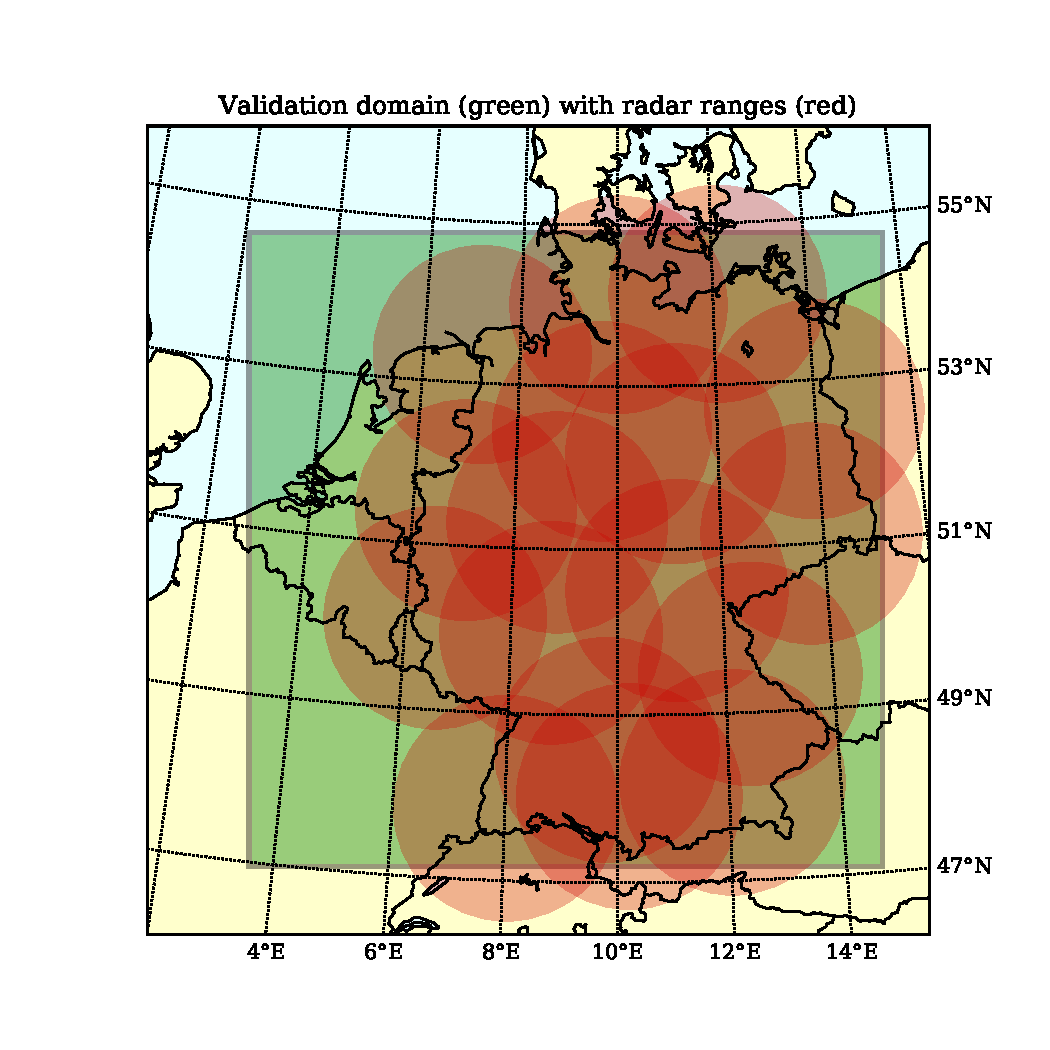
\includegraphics[width=0.8\textwidth]{Grafiken/Abbildungen/radolan_domain.pdf}
\caption{Map of the validation domain (green) with the ranges of the weather radars of the German weather radar network (red). The validation domain is the standard domain of the German weather radar network as defined in \citet{RADOLANkurz2018} and it comprises an area of \SI{900 x 900}{\kilo\metre} covering Germany and parts of its neighbouring countries.}
\label{fig:radolan_domain}
\end{figure}

\section{Case days}
In the validation study of the NWC\,SAF CI product v2016 by \citet{Karagiannidis2016}, four case days have been considered to validate the product: 25\textsuperscript{th} May 2010, 28\textsuperscript{th} June 2010, 2\textsuperscript{nd} July 2010 and 3\textsuperscript{rd} July 2010. To ensure consistency, three of the four case days are used. As there was no convective development over Germany for 28\textsuperscript{th} June 2010, this day is not considered here. In order to extend the basis for validation, three additional case days were added: 23\textsuperscript{rd} May 2012, 18\textsuperscript{th} June 2013 and 20\textsuperscript{th} June 2013. A synoptic overview of the three additional case days is given below. For a synoptic description of the other three case days, please refer to \citet{Karagiannidis2016}.

\subsection{23\textsuperscript{rd} May 2012}
On 23\textsuperscript{rd} May 2012 large parts of Western and Central Europe are influenced by a pronounced high pressure ridge which extends from the Iberian peninsula until the Baltic Sea (Fig. \ref{fig:23052012_500hpa}). Corresponding to the high pressure ridge in the middle troposphere a ground high pressure system is located over Scandinavia (Fig.~\ref{fig:synoptik_20120523}(a)). Over the eastern Atlantic ocean a quite distinct height trough expands from Iceland to the south with several corresponding low pressure systems at the ground. This large scale weather pattern leads to a north eastern flow towards Central Europe. 

Looking at the surface pressure chart (Fig.~\ref{fig:synoptik_20120523}(b)) it can be seen, that the pressure gradients are relatively low over Western and Central Europe but are stronger along the coasts of the Northern and Baltic Sea along the frontal zone. 

Concerning the GFS reanalysis charts for the KO index / vertical movement (Fig.~\ref{fig:synoptik_20120523}(c)) and LI/ CAPE (Fig.~(d)), it has to be noted that the atmospheric composition is quite unstable which can be seen from the strongly negative values of the KO index. Moreover there are large areas in Central Europe with strong vertical movement induced by the rather high temperatures of the day. Especially over Northern Germany the CAPE is moderately elevated and the LI shows high values, which both indicates a high potential for convective development.

\begin{figure}[htbp]
	\centering
	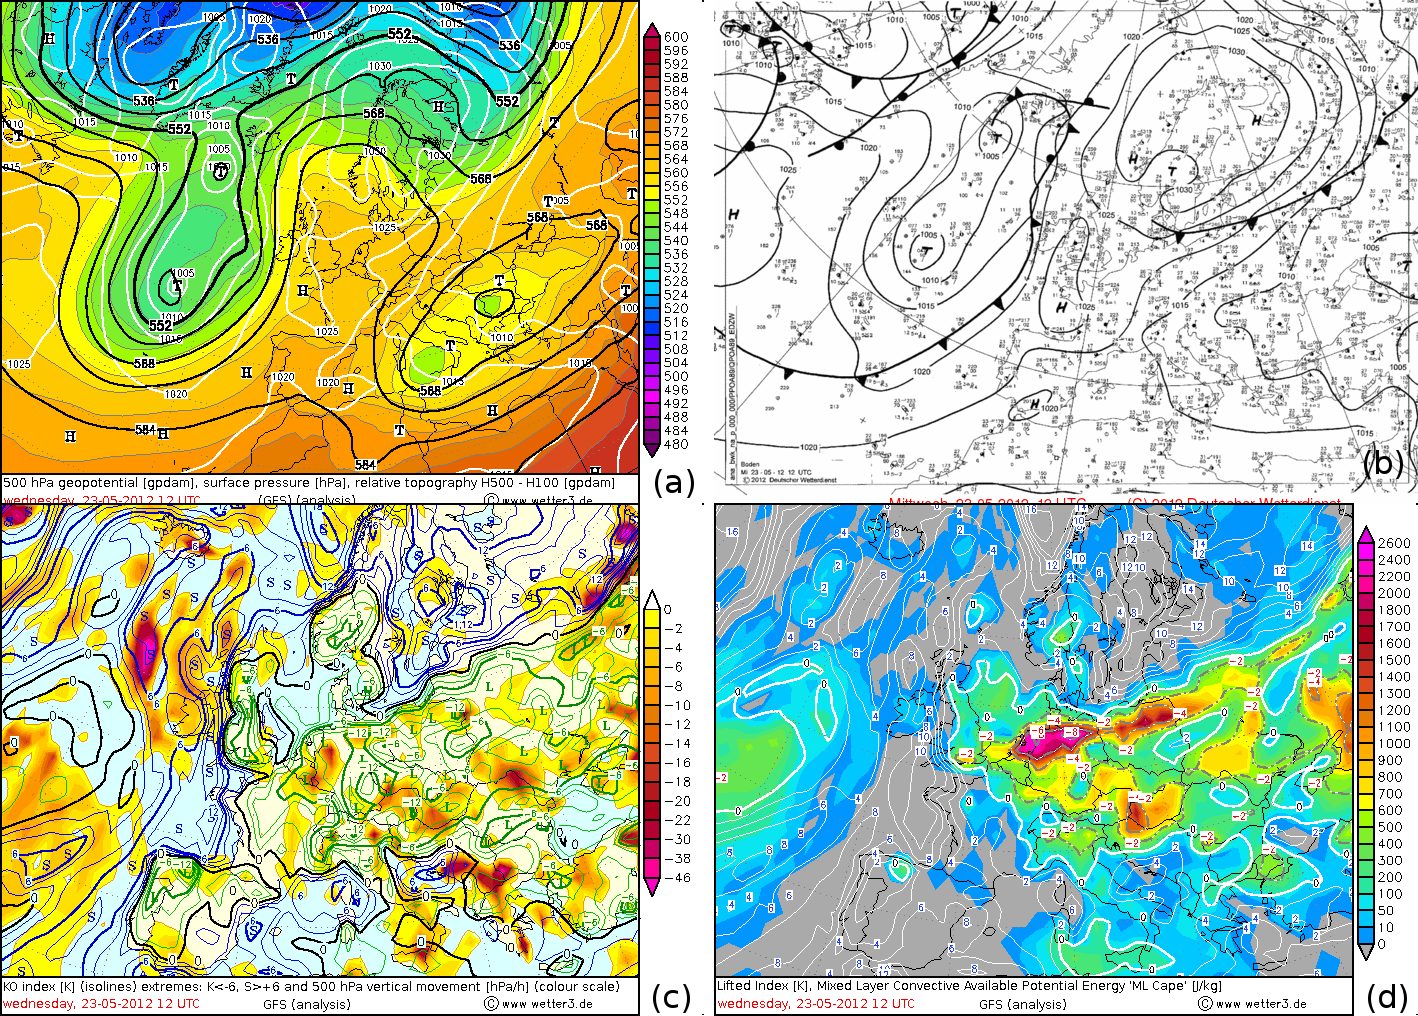
\includegraphics[width=\linewidth]{Grafiken/Abbildungen/synoptik_20120523.png}
	\caption{Synoptic overview for 23\textsuperscript{rd} May 2012, 12:00 UTC, (a) \SI{500}{\hecto\pascal} geopotential, surface pressure and relative topography \SI{500}{\hecto\pascal} - \SI{1000}{\hecto\pascal}, source: www.wetter3.de, (b) Surface pressure analysis, source: Deutscher Wetterdienst, (c) KO index and \SI{500}{\hecto\pascal} vertical movement, source www.wetter3.de, (d) Lifted Index and Mixed Layer Convective Available Potential Energy, source: www.wetter3.de}
    \label{fig:synoptik_20120523}  
\end{figure}

\subsection{18\textsuperscript{th} June 2013}
On 18\textsuperscript{th} June 2013 the weather over Central Europe was dominated by a upper level high pressure ridge which extended from Northern Africa to South West and Central Europe while a upper level trough expanded from Iceland south to the Iberian peninsula where a higher level low pressure core was situated (Fig.~ \ref{fig:synoptik_20130618}(a)). This large scale weather pattern lead to a southern flow to Central Europe. Along the frontal zone of the upper level low pressure system, hot and unstable air masses where transported northwards leading to an unstable atmospheric composition and a pronounced heat wave over south western Central Europe.

In the ground pressure field several smaller low pressure systems are located below the upper level high pressure ridge, also leading to an unstable atmospheric composition (Fig.~\ref{fig:synoptik_20130618}(b)). 

The KO index / vertical movement chart (Fig.~\ref{fig:synoptik_20130618}(c)) shows strong vertical movements over South West and Central Europe while the KO index is only slightly negative, indicating only a slightly unstable atmosphere. The LI / CAPE chart (Fig.~\ref{fig:synoptik_20130618}(d)) shows, that strongly elevated CAPE and also strongly negative LI values are present over Central Europe, indicating a strong potential for convective development.

\begin{figure}[htbp]
	\centering
	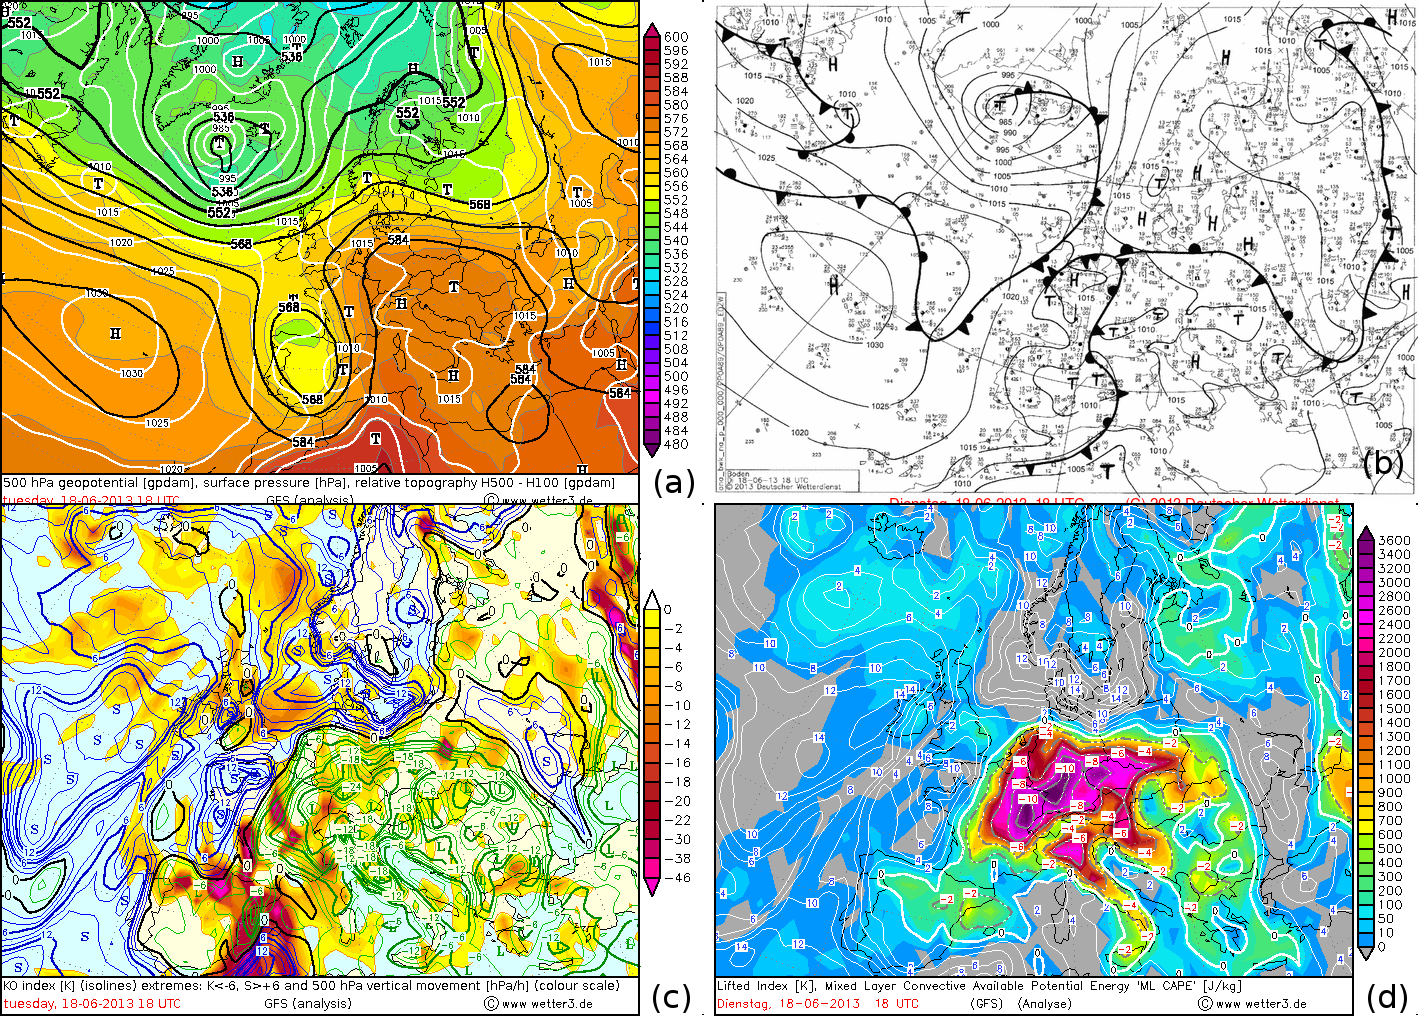
\includegraphics[width=\linewidth]{Grafiken/Abbildungen/synoptik_20130618.png}
	\caption{Same as Fig.~\ref{fig:synoptik_20120523} but for 18\textsuperscript{th} June 2013, 12:00 UTC}
    \label{fig:synoptik_20130618}  
\end{figure}


\subsection{20\textsuperscript{th} June 2013}
The weather situation of the 20\textsuperscript{th} June 2013 was quite similar to the one on 18\textsuperscript{th} June 2013. The large scale weather pattern is similar but the higher level low pressure core situated over Southern France gained more influence on the weather in Central Europe (Fig.~\ref{fig:synoptik_20130620}(a)). Additionally a heat low pressure system formed in the hot air over North Eastern Germany with a convergence line on its western boundary as can be seen in the ground pressure field (Fig.~\ref{fig:synoptik_20130620}(b)). Along this convergence line several thunderstorms formed and in the evening the cold front of the low pressure system over Southern France reached Germany leading to the formation an organised thunderstorm line.

The KO index / vertical movement chart (Fig.~\ref{fig:synoptik_20130620}(c)) shows strong vertical movements over North West Germany and also a strongly negative KO index over this area, indicating a quite unstable atmosphere. The LI / CAPE chart (Fig.~\ref{fig:synoptik_20130620}(d)) shows, that strongly elevated CAPE and also strongly negative LI values are present over the most parts of Germany, indicating a strong potential for convective development.

\begin{figure}[htbp]
	\centering
	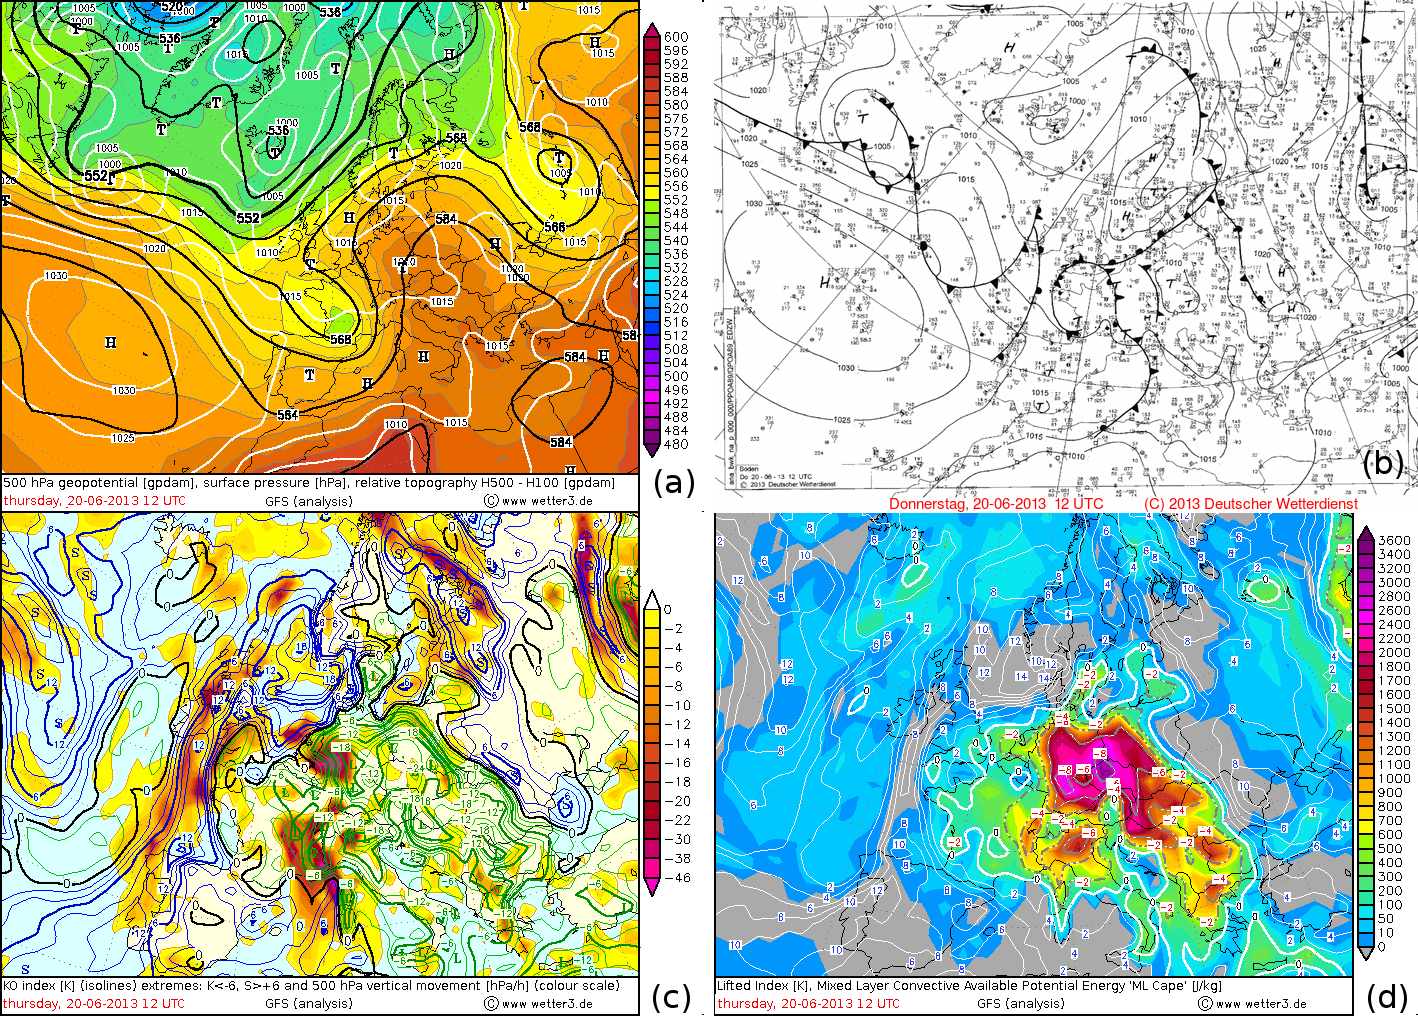
\includegraphics[width=\linewidth]{Grafiken/Abbildungen/synoptik_20130620.png}
	\caption{Same as Fig.~\ref{fig:synoptik_20120523} but for 20\textsuperscript{th} June 2013, 12:00 UTC}
    \label{fig:synoptik_20130620}  
\end{figure}

\section{Definition of Ground Truth}
\label{sec:haci}
Using the RADOLAN RX composite, isolated convective objects have been identified using the method described in \citet{Haberlie_2015}. First the radar data (Fig. \ref{fig:haberlie}(a)) has been masked using a reflectivity factor threshold of \SI{35}{\dbZ} (Fig. \ref{fig:haberlie}(b)) to delineate convectively active regions. These regions are then grouped into objects by requiring connectivity. A buffer mask is generated around existing objects as well as the border of the radar range using a buffer radius of \SI{15}{\kilo\metre}. This buffer mask is applied to the next time step, in order to identify newly developing convective objects (Fig. \ref{fig:haberlie}(c)). Finally, all newly developed convective objects outside the buffer mask with a reflectivity factor of over \SI{35}{\dbZ} are considered as new convective objects, which have thus initiated within the last five minutes (Fig. \ref{fig:haberlie}(d)). Requiring a minimum object life time of \SI{30}{\minute} together with some additional  criteria, only objects are retained which have a sufficient life time to be considered as convective objects (Fig. \ref{fig:haberlie}(e)). Convective object identificaiton is done at five minutes time resolution for all case days, and is subsequently aggregated to \SI{15}{\minute} time steps to match the temporal resolution of the NWCSAF CI product. These object represent the ground truth used further for the validation of the CI product.

\begin{figure}[htbp]
\centering
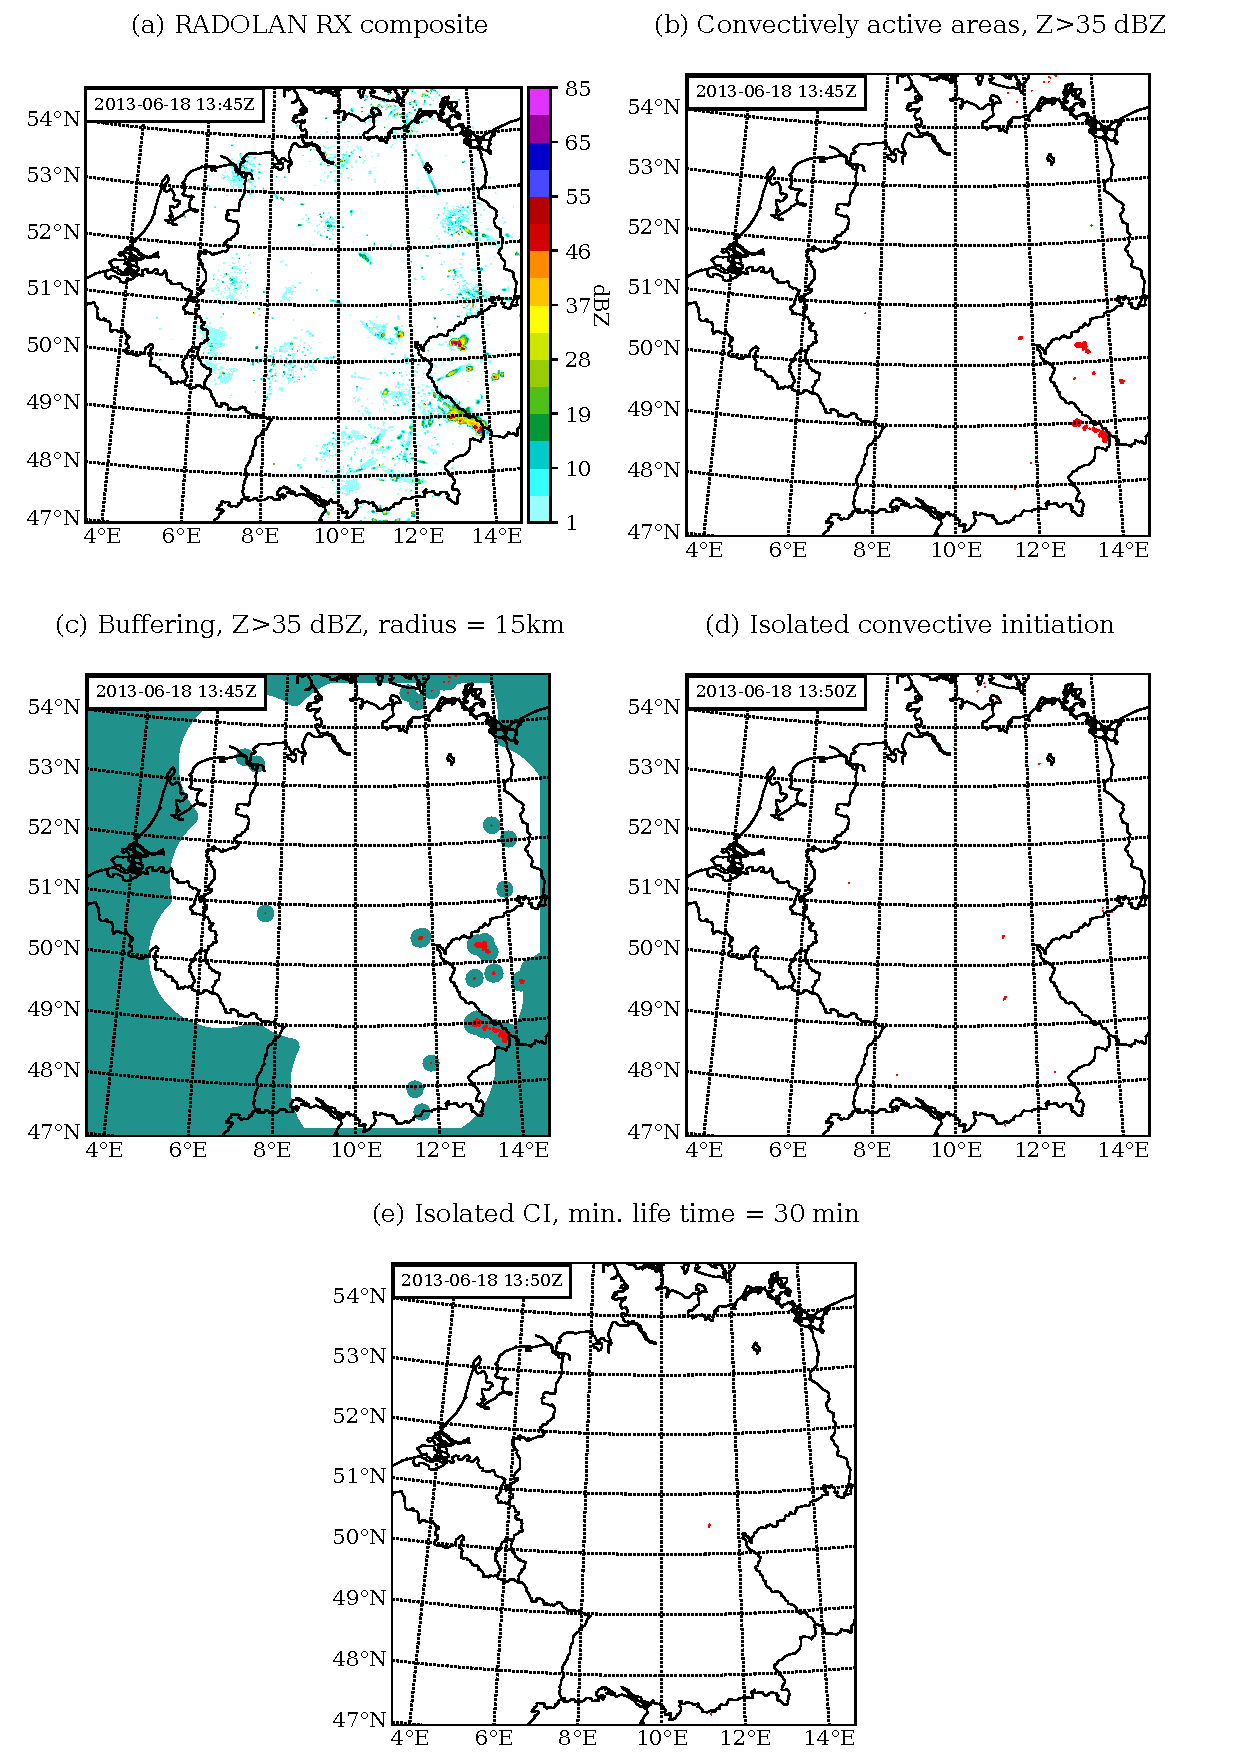
\includegraphics[height=\textheight]{Grafiken/Abbildungen/haberlie_prinzip.pdf}
\caption{Principle of deriving the ground truth. Using weather radar data (a), the data are masked using a reflectivity threshold of \SI{35}{\dbZ} to derive convectively active areas (b). Then these objects are buffered using a buffer radius of \SI{15}{\kilo\metre} (c). Using these buffers the, data of the next time step is masked, so that only isolated newly developing convection is taken into account (d). After that, to only consider precipitating objects with an adequate life  time, all objects with a minimum life time below \SI{30}{min} are masked out (e).}
\label{fig:haberlie}
\end{figure}

It has to be noted that this definition of ground truth is rather strict and quite different from the approach chosen by \citet{Karagiannidis2016}. Hence, a second definition of ground truth is also considered for improved comparability. This ground truth is also based on the RADOLAN RX radar composite, which is only masked with a reflectivity factor of \SI{30}{\dbZ}, considering all regions exceeding this radar reflectivity as ground truth.

\section{Derivation of motion fields}
The motion of cloud fields in the satellite observations was estimated using the implementation of the TV-L1 optical flow algorithm proposed by \citet{Zach2007}. The Python interface to the OpenCV library \citep{opencV_library} has been used heere. The algorithm parameters where optimized using the MPI Sintel test dataset \citep{Butler:ECCV:2012}, and are given in Tab. \ref{tab:oflow}. Motion fields have been calculated from Meteosat's IR \SI{10.8}{\micro\metre} and HRV channels considering \SI{15}{\minute} time steps. The TV-L1 optical flow approach differs from the cross correlation-based approach by \citet{MecikalskiBedka2006} to derive atmospheric motion vectors (AMV) by allowing discontinuities in the flow field, and tends to be more robust against noise than other techniques of motion tracking \citep{Perez2013}.

\begin{table}[htb]
\caption{opencv parameters used for the estimation of the optical flow using the method proposed \citet{Zach2007}}
\begin{tabular}{llS} 
\toprule
parameter & description & {value}\\ 
\midrule 
$\epsilon$ & stopping criterion threshold used in the numerical scheme & \num{0.01}\\ 
$\gamma$ & coefficient for additional illumination variation term & 0.4\\ 
$\lambda$ & weight parameter for the data term, attachment parameter & 0.2\\ 
$\mu$ & kernel size of the median filter & 1\\ 
$\tau$ & time step of the numerical scheme & 0.25\\ 
$\theta$ & Weight parameter for (u - v)\textsuperscript{2}, tightness parameter & 0.8\\ 
$\mathrm{N}_\mathrm{inner}$ & number of inner iterations  used in the numerical scheme & 7\\ 
$\mathrm{N}_\mathrm{outer}$ & number of outer iterations  used in the numerical scheme & 40\\ 
$\mathrm{N}_\mathrm{scales}$ & number of scales used to create the pyramid of images & 5\\ 
$\mathrm{S}_\mathrm{scales}$ & steps between scales & 0.5\\
$\mathrm{N}_\mathrm{warp}$ & number of warpings per scale & 5\\ 
\addlinespace
\bottomrule
\end{tabular}
\label{tab:oflow}
\end{table}

\section{Cloud objects}
\label{sec:cloud}
To validate the detections of the NWC\,SAF CI product and the detections of the radar based approach presented above, cloud objects have been derived. 

The cloud objects are based on the NWC\,SAF cloud mask product and the MSG HRV channel, as its higher spatial resolution allows for a better separability of cloud objects than the standard MSG resolution. As the HRV channel is in the visible spectrum, and so there is no data for the night time, only a time frame of twelve hours centered around noon CET (05:00 am UTC to 05:00 pm UTC) has been chosen for the derivation of cloud objects. This time frame has the advantage that there is data for all case days and it also avoids the time around sunrise and sunset where atmospheric scattering effects make the data not usable for our objective.

For the derivation of meaningful cloud objects, the rather high HRV spatial resolution also has the drawback that often very small non-convective clouds are derived as cloud objects leading to an artificially high rate of missed detections. To overcome this, the HRV field (Fig.~\ref{fig:hrv_seg}(a)) was filtered using a Gaussian filter (Fig.~\ref{fig:hrv_seg}(b)) and the objects were derived from the smoothed HRV field ((Fig.~\ref{fig:hrv_seg} (c) and (d)). Additionally a minimum size an object has to have to be considered was set. To find suitable filter, minimum size and threshold parameters, a number of different parameters combination has been tested against the overlap size of ground truth objects and cloud objects for the 25\textsuperscript{th} May 2010. The result of the analysis is shown in Fig. \ref{fig:filter-parameters}. It turns out, that the two parameters with the highest impact on the overlap size are the size of the Gaussian kernel and the threshold used to define which parts of the HRV channel field are objects. The minimum size of the objects and the connectivity used to segment the objects does not seem to have a large influence. The maximum intersection size between ground truth and cloud objects can be achieved by a rather strong smoothing, setting the Gaussian filter parameter $\sigma$ to three, and setting the HRV threshold to \num{0.3}. Additionally, for the derivation of the cloud objects, to avoid to small objects, the minimum object size was set to \num{10}  and the connectivity type to \num{8} neighbours. 
 
\begin{figure}[htbp]
\centering
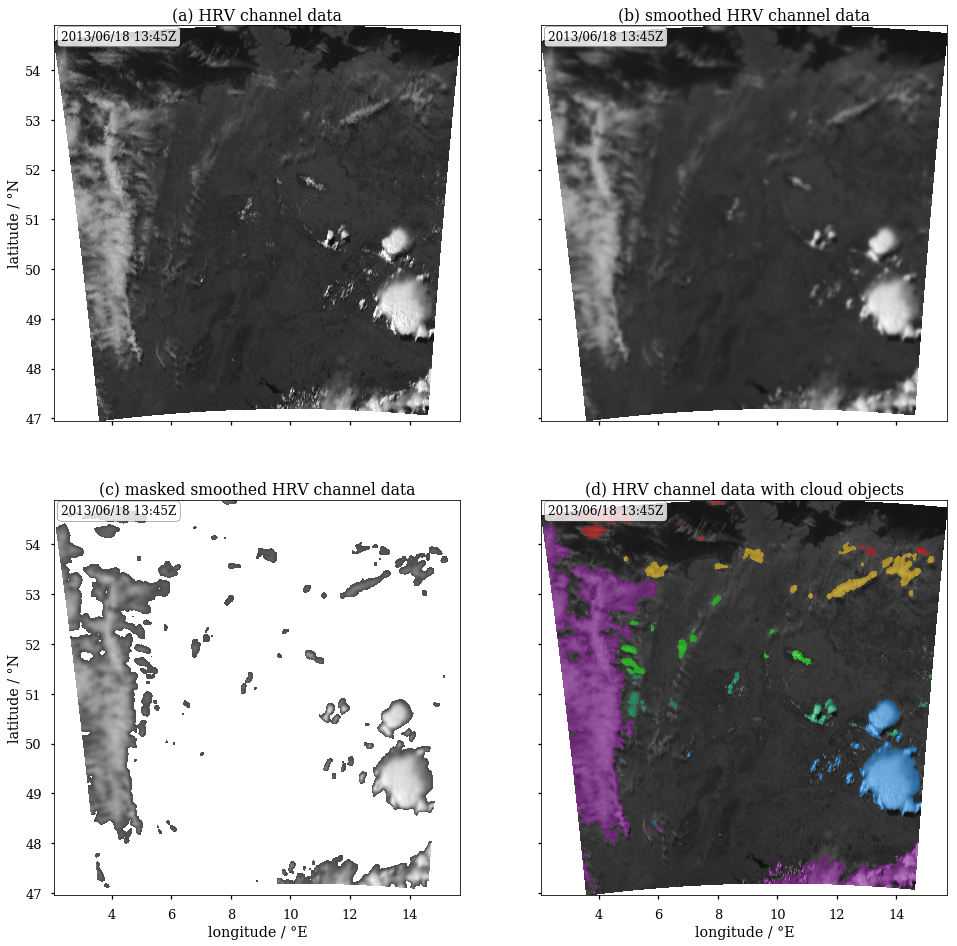
\includegraphics[width=\textwidth]{Grafiken/Abbildungen/wolkenobjektprinzip.png}
\caption{Principle of deriving the cloud objects. Using HRV channel data (a), the data are smoothed using a Gaussian blur filter with a $\sigma$ value of 3 (b). Then these objects are buffered using a buffer radius of \SI{15}{\kilo\metre} (c). Using these buffers the, data of the next time step is masked, so that only isolated newly developing convection is taken into account (d). After that, to only consider precipitating objects with an adequate life  time, all objects with a minimum life time below \SI{30}{min} are masked out (e).}
\label{fig:hrv_seg}
\end{figure}

\begin{figure}[htbp]
\centering
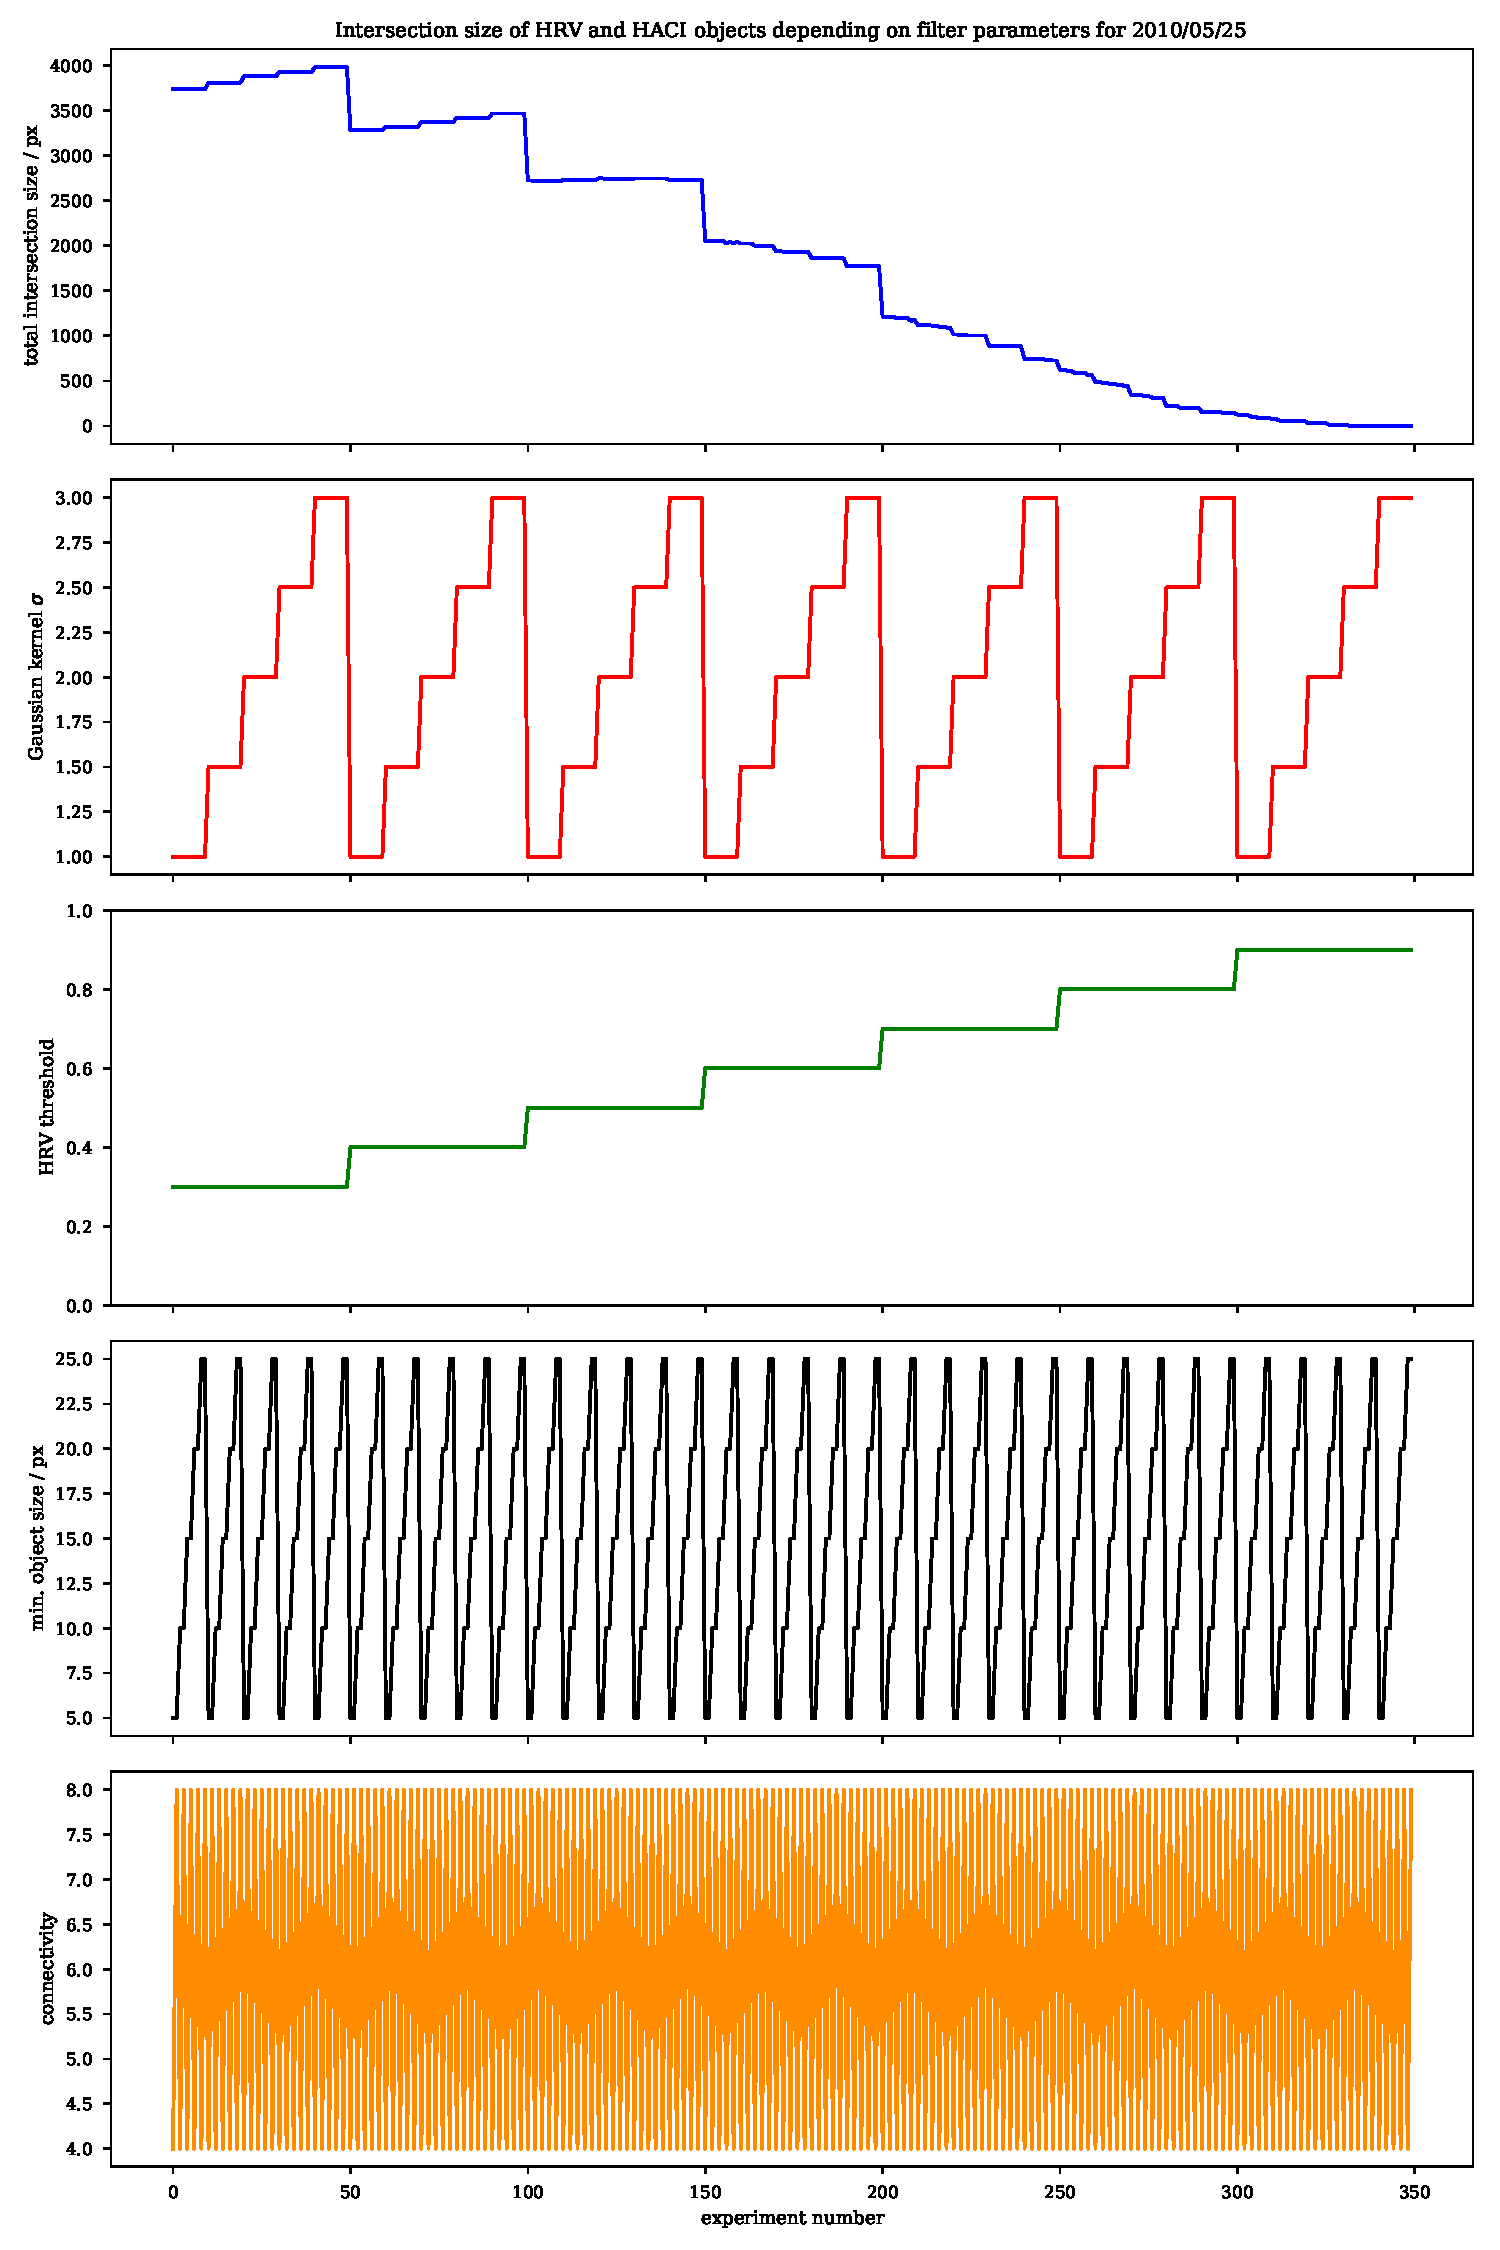
\includegraphics[height=\textheight]{Grafiken/Abbildungen/parameter_plot.pdf}
\caption{Intersection size between cloud and ground truth objects for a number of filter and segmentation parameters.}
\label{fig:filter-parameters}
\end{figure}

Objects tracks are created using the motion fields derived from the MSG HRV channel applying an overlap tracking approach. Starting from the first emergence of the particular object, the object is moved forward in time using the motion field. If the objects of the first and second time step overlap, an object path is created for the two time steps and so on. As the object structure often is quite complex with many splits and merges, mathematical graphs have been created to allow for an analysis of the object structure. Using the graphs, only single cell objects the part of the object tracks prior to splits and merges have been used in the further analysis. To allow for a comparison with the radar data, the tracks also have been parallax corrected using the cloud top height of the NWC\,SAF cloud height product.

To be consistent with the ground truth definition, only objects with a minimum life time of \SI{30}{\minute} have been considered in the further analysis.

\section{Validation approach}
\label{sec:validation}
The validation of the NWC\,SAF CI product detections is based on cloud objects derived from MSG HRV data and weather radar detections as ground truth.

As shown in Fig. \ref{fig:schema}, the validation strategy is based on the intersection of cloud objects, CI detections and ground truth objects. Given a track of a cloud object the cloud object is considered to be detected by the NWC\,SAF CI product if there is an intersection between the cloud object and pixels with a CI probability of larger than \SI{0}{\percent}. If there is an intersection between the cloud object and pixels with different CI probabilities for one time step, only the highest CI probability is counted, and if there are more than one intersections of the cloud object and CI pixels along the object track, only the first intersection time step is counted. 

In the next step, starting from the CI detection time step, it is checked if there is an intersection between the cloud object and a ground truth object within the next \SI{30}{\minute}. If necessary, the track is getting extended by propagating the last available track point forward in time using the motion fields. If an intersection between a detected cloud object and a ground truth object can be observed within the next \SI{30}{\minute} it is counted as a true positive case for the highest CI probability level of the detection time step. If not, than it is counted as a false positive case.

If there are intersections with at least one ground truth object along the cloud object track and there are no intersections with CI pixels or the intersection with the first intersection with a ground truth object is earlier than the first intersection with CI pixels, the case is counted as false negative.

If a cloud object neither intersects with CI pixels nor with a ground truth objects it is counted as true negative.

This leads to the confusion matrix given in Tab. \ref{tab:confusion}.

\begin{figure}[htbp]
\centering
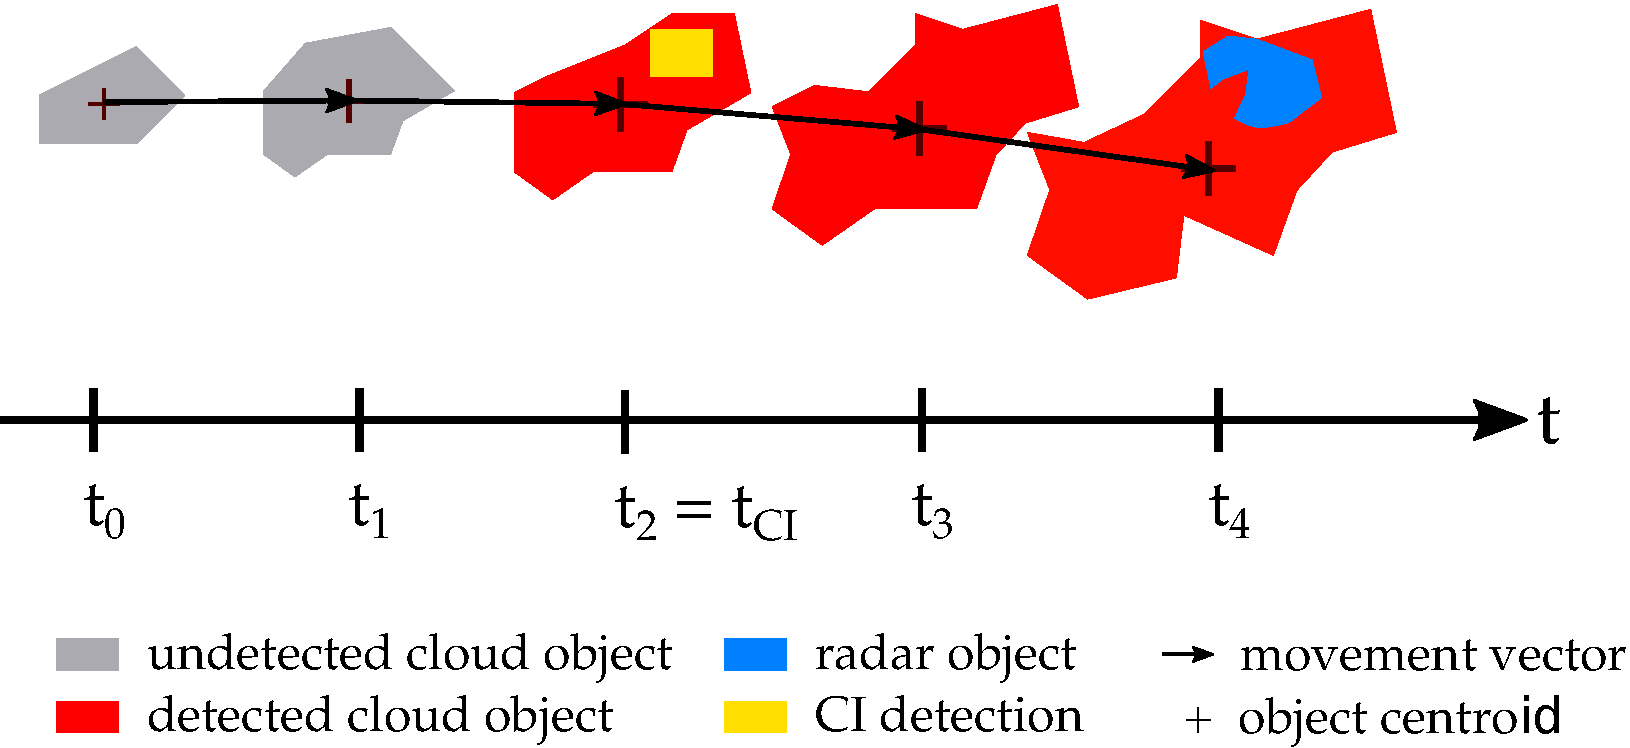
\includegraphics[width=0.7\textwidth]{Grafiken/Abbildungen/verification_scheme_new.pdf}
\caption{Schematic of the validation approach. Starting from a cloud object (red) a cloud object track is created (denoted by the vector arrows) and a validation area is spanned around the object centroids (grey circles). If a CI object (yellow) is inside the validation area a new object track with validation region is created. If a radar object (green) is detected inside the new \SI{30}{\minute} validation area the cloud object is counted as a true positive}
\label{fig:schema}
\end{figure}

\begin{table}[htb]
\centering
\caption{Confusion matrix for the validation}
\begin{tabular}{cccc} 
\toprule
\multirow{2}{*}{CI product detection} &     & \multicolumn{2}{c}{weather radar detection} \\
							   						  \cmidrule{3-4}
									  &     & yes   		   & no \\
\midrule
\multirow{2}{*}{CI level 1 detected}  & yes & true positive, TP$_\text{CI level 1}$  & false positive, FP$_\text{CI level 1}$ \\
	                                  & no  & false negative, FN$_\text{CI level 1}$  & true negative, TN$_\text{CI level 1}$ \\ 
\multirow{2}{*}{CI level 2 detected}  & yes & true positive, TP$_\text{CI level 2}$  & false positive, FP$_\text{CI level 2}$ \\ 
	                                  & no  & false negative, FN$_\text{CI level 2}$  & true negative, TN$_\text{CI level 2}$ \\ 
\multirow{2}{*}{CI level 3 detected}  & yes & true positive, TP$_\text{CI level 3}$  & false positive, FP$_\text{CI level 3}$ \\ 
	                                  & no  & false negative, FN$_\text{CI level 3}$  & true negative, TN$_\text{CI level 3}$ \\ 
\multirow{2}{*}{CI level 4 detected}  & yes & true positive, TP$_\text{CI level 4}$  & false positive, FP$_\text{CI level 4}$ \\ 
	                                  & no  & false negative, FN$_\text{CI level 4}$  & true negative, TN$_\text{CI level 4}$ \\
\addlinespace
\bottomrule
\end{tabular}
\label{tab:confusion}
\end{table}

For the assessment of the validation, several metrics can be derived from the confusion matrix. In this study the following are used:

\begin{itemize}
\item Probability Of Detection $\mathrm{POD} = \frac{\mathrm{TP}}{\mathrm{TP} + \mathrm{FN}}$, which is the probability to detect an event
\item False Alarm Rate $ \mathrm{FAR} = \frac{\mathrm{FP}}{(\mathrm{FP} + \mathrm{TN})} $, which is the probability to detect an event where there is no event
\item Heidke Skill Score \citep{Heidke1926}$ \mathrm{HSS} = \frac{2 (\mathrm{TP} \cdot \mathrm{TN}) - \mathrm{FP} \cdot \mathrm{FN}}{ (\mathrm{TP} + \mathrm{TF}) (\mathrm{FN} + \mathrm{TN}) (\mathrm{FP} + \mathrm{TN})}$, which is a measure of how good is the algorithm performance against a detection by chance
\item Critical Sucess Index $ \mathrm{CSI} = \frac{\mathrm{TP}}{\mathrm{TP} + \mathrm{FN} + \mathrm{FP}}$, which is a measure of how well forecasts events correspond to observed events 
\end{itemize}